\chapter{Практическая часть}

\section{Генерация трёхмерной сетки с ячейками в виде шестигранников}

При написании программы был использован следующий подход к построению сетки на шестигранных элементах.\\
\texttt{\hspace*{0.5em}1. [lines amount x] 2 [lines amount y] 2 [lines amount z] 2\\}
\texttt{\hspace*{0.5em}2. [field description of points]\\}
\texttt{\hspace*{0.5em}3. 0.0 0.0 0.0 \qquad 1.0 0.0 0.0\\}
\texttt{\hspace*{0.5em}4. 0.0 1.0 0.0 \qquad 1.0 1.0 0.0\\}
\texttt{\hspace*{0.5em}5. 0.0 0.0 1.0 \qquad 1.0 0.0 1.0\\}
\texttt{\hspace*{0.5em}6. 0.0 1.0 1.0 \qquad 1.0 1.0 1.0\\}	
\texttt{\hspace*{0.5em}7. [unique areas amount] 1\\}
\texttt{\hspace*{0.5em}8. [unique areas description]\\}
\texttt{\hspace*{0.5em}9. 1 0 1 0 1 0 1\\}
\texttt{10. [unique areas coefficients description]\\}
\texttt{11. 1 1.0 1.0\\}
\texttt{12. [delimiters above X description] 1 1.0\\} 
\texttt{13. [delimiters above Y description] 3 1.1\\}
\texttt{14. [delimiters above Z description] 4 0.8\\}
\texttt{15. [borders amount] 6\\}
\texttt{16. [borders description]\\}
\texttt{17. 1 1 0 1 0 0 0 1\\}
\texttt{18. 1 1 0 1 1 1 0 1\\}
\texttt{19. 1 1 0 0 0 1 0 1\\}
\texttt{20. 1 1 1 1 0 1 0 1\\}
\texttt{21. 1 1 0 1 0 1 0 0\\}
\texttt{22. 1 1 0 1 0 1 1 1\\}

В первой строке заданы количество опорных узлов $N_x^W, \,N_y^W, \,N_z^W,$ базовой плоскости по осям $X,\,Y,\,Z$ соответственно. С третьей по шестую строки перечисленны тройки чисел $\left(x_i, \, y_i, \, z_i\right)$ - как раз и определяющие эти опорные узлы. 

В седьмой строке указано количество уникальных областей в расчётной области, которые имеют определённые уникальные значения физических параметров $\mu$ и $\sigma$. Начиная с девятой строки (в общем случае должен быть построчный перечень каждой области) описывается геометрическое расположение $i$ - ой области.  В одиннадцатой строке указаны уникальные значения параметров $\mu$ и $\sigma$ для $i$ - ой области.

В строках с двенадцатой по четырнадцатую описывается количество и характер необходимых разбиений для осей $X,\,Y,\,Z$ соответственно.

В пятнадцатой строке целочисленным значением задаётся количество границ. Далее с семнадцатой по двадцать вторую строки описывается расположение и характер этих границ. Первым числом задаётся тип краевого условия (т.е. принимает значения 1 или 2), вторым числом задаётся номер формулы, третьим первая координатная линия по оси $X$, четвёртым вторая координатная линия по оси $X$, пятым и шестым аналогично по оси $Y$ и седьмым и восьмым по оси $Z$.

Пример расчётной области этой фигуры изображён на рисунке (\ref{fig:ExampleCube}).

\begin{figure}
	\centering
	\vspace*{0.7cm}
	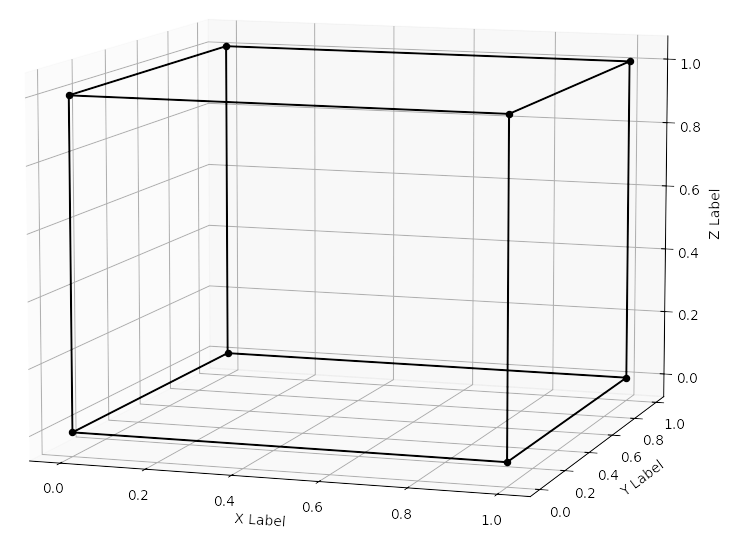
\includegraphics[width=0.7\linewidth]{images/ExampleCube.png}
	\caption{Расчетная область для кубика}
	\label{fig:ExampleCube}
\end{figure}

Попробуем подробить расчётную область (\ref{fig:ExampleCube}) на несколько частей. Получим сетку изображённую на рисунке (\ref{fig:GridCube}).

\begin{figure}
	\centering
	\vspace*{0.7cm}
	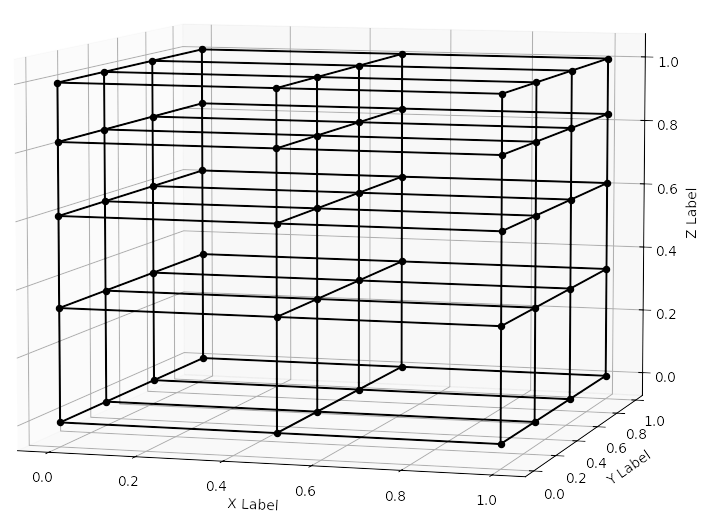
\includegraphics[width=0.7\linewidth]{images/GridCube.png}
	\caption{Секта для кубика}
	\label{fig:GridCube}
\end{figure}

Приведём ещё насколько примеров для построения сеток на шестигранниках, изображённых на рисунках  \ref{fig:Emerald} - \ref{fig:DEmerald}.

\begin{figure}
	\begin{minipage}[h]{0.49\linewidth}
		\center{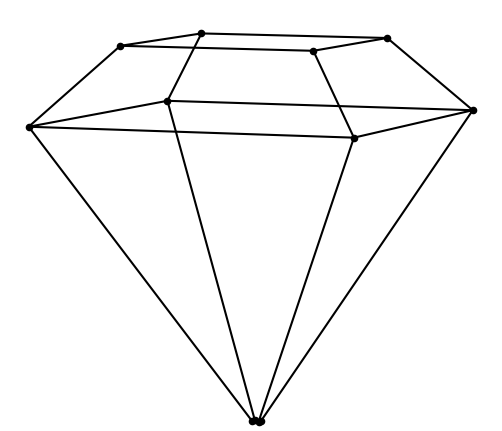
\includegraphics[width=0.5\linewidth]{images/EmeraldField.png} \\ а)}
	\end{minipage}
	\hfill
	\begin{minipage}[h]{0.49\linewidth}
		\center{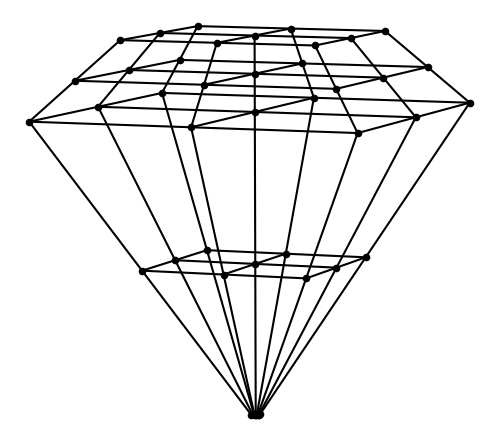
\includegraphics[width=0.5\linewidth]{images/EmeraldMesh.png} \\ б)}
	\end{minipage}
	\caption{Расчётная область в форме изумруда (а) и сетка к ней (б).}
	\label{fig:Emerald}
\end{figure}

\begin{figure}
	\begin{minipage}[h]{0.49\linewidth}
		\center{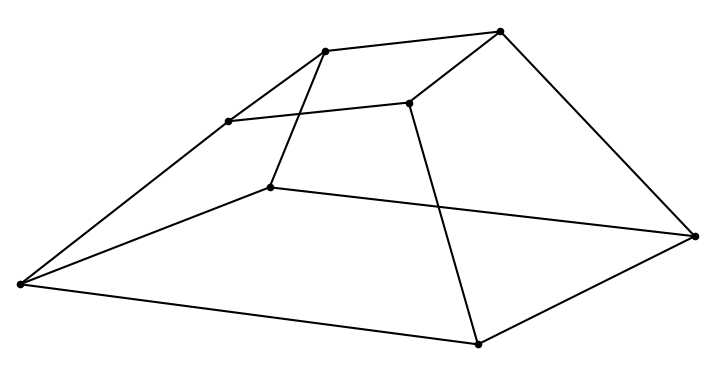
\includegraphics[width=0.5\linewidth]{images/PyramidField.png} \\ а)}
	\end{minipage}
	\hfill
	\begin{minipage}[h]{0.49\linewidth}
		\center{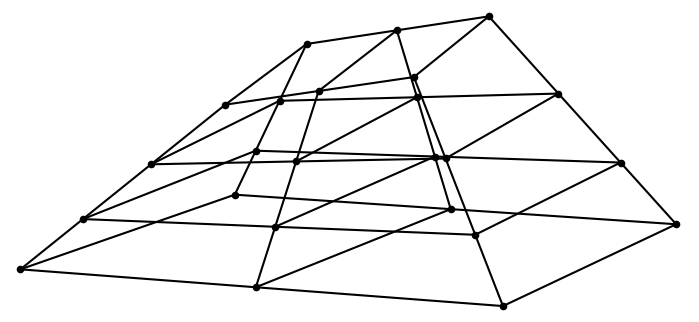
\includegraphics[width=0.5\linewidth]{images/PyramidMesh.png} \\ б)}
	\end{minipage}
	\caption{Расчётная область в форме скошенной пирамиды (а) и сетка к ней (б).}
	\label{fig:Pyramid}
\end{figure}

\begin{figure}
	\begin{minipage}[h]{0.49\linewidth}
		\center{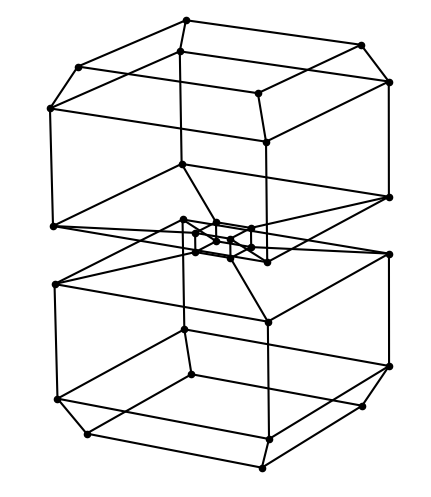
\includegraphics[width=0.5\linewidth]{images/HGField.png} \\ а)}
	\end{minipage}
	\hfill
	\begin{minipage}[h]{0.49\linewidth}
		\center{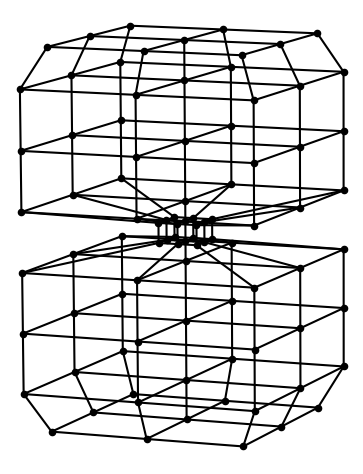
\includegraphics[width=0.5\linewidth]{images/HGMesh.png} \\ б)}
	\end{minipage}
	\caption{Расчётная область в форме песочных часов (а) и сетка к ней (б).}
	\label{fig:HG}
\end{figure}

\begin{figure}
	\begin{minipage}[h]{0.49\linewidth}
		\center{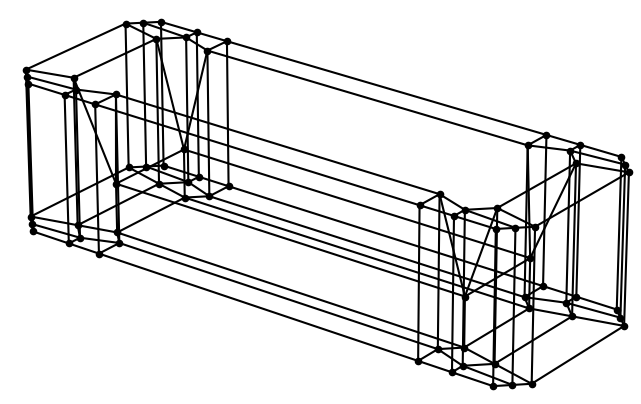
\includegraphics[width=0.5\linewidth]{images/BathField.png} \\ а)}
	\end{minipage}
	\hfill
	\begin{minipage}[h]{0.49\linewidth}
		\center{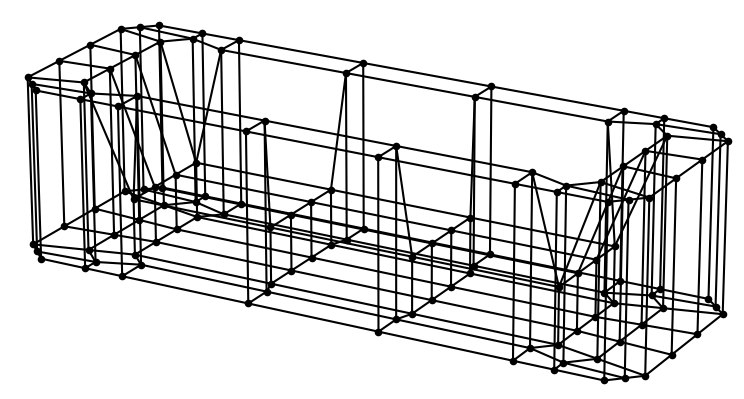
\includegraphics[width=0.5\linewidth]{images/BathMesh.png} \\ б)}
	\end{minipage}
	\caption{Расчётная область в форме ванной (а) и сетка к ней (б).}
	\label{fig:Bath}
\end{figure}

\begin{figure}
	\begin{minipage}[h]{0.49\linewidth}
		\center{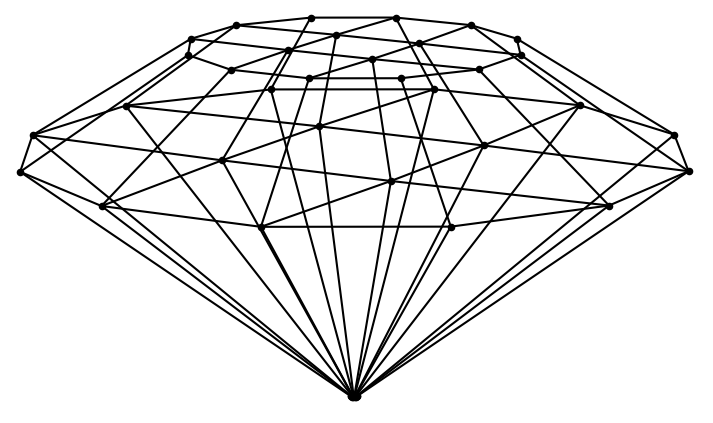
\includegraphics[width=0.5\linewidth]{images/DEmeraldField.png} \\ а)}
	\end{minipage}
	\hfill
	\begin{minipage}[h]{0.49\linewidth}
		\center{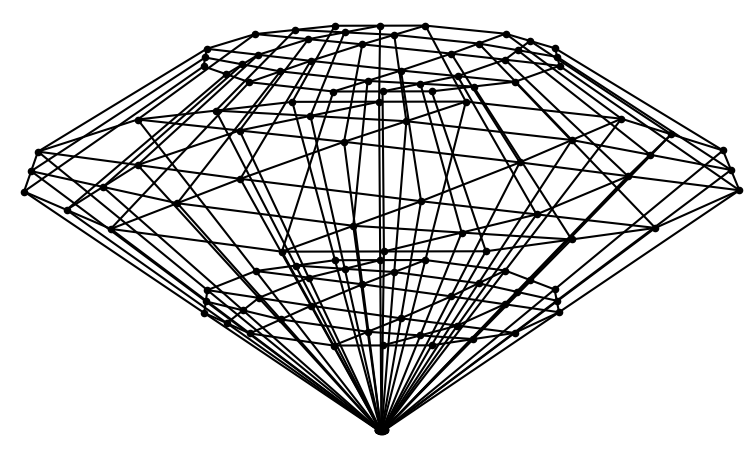
\includegraphics[width=0.5\linewidth]{images/DEmeraldMesh.png} \\ б)}
	\end{minipage}
	\caption{Расчётная область в форме детализированного изумруда (а) и сетка к ней (б).}
	\label{fig:DEmerald}
\end{figure}

Таким образом, программа для построения сетки может строить достаточно геометрически сложные фигуры.

\section{Численное интегрирование}

При расчёте элементов локальных матриц жёсткости (\ref{eq_1_11}) и масс (\ref{eq_1_12}) будем использовать численное интегрирование методами Гаусса разных порядков (2, 3, 4, 5). Результаты численного интегрирования на некоторых функциях приведены в таблицах \ref{tab:numIntegr1} - \ref{tab:numIntegr7}. Область интегрирования для всех функций единый: $\Omega_E \in \left[-1; 1\right]_x \cross \left[-1; 1\right]_y \cross \left[-1; 1\right]_z$.

\begin{table}
	\caption{Тестирование численного интегрирования на функции $u = 2$.}
	\centering
	\small
	\begin{tabularx}{1.0\textwidth}{| >{\raggedright\arraybackslash}X | >{\raggedright\arraybackslash}X | >{\raggedright\arraybackslash}X |>{\raggedright\arraybackslash}X |>{\raggedright\arraybackslash}X |}
		\hline
		\centering{Аналитический результат} & \centering{Гаусс 2} & \centering{Гаусс 3} & \centering{Гаусс 4} & \centering{Гаусс 5} \tabularnewline \hline
		
		\centering{16.0} & \centering{1.6000000e+01}& \centering{1.6000000e+01} & \centering{1.6000000e+01} & \centering{1.6000000e+01} \tabularnewline \hline
		
	\end{tabularx}
	\label{tab:numIntegr1}
\end{table}


\begin{table}
	\caption{Тестирование численного интегрирования на функции $u = x + y + z$.}
	\centering
	\small
	\begin{tabularx}{1.0\textwidth}{| >{\raggedright\arraybackslash}X | >{\raggedright\arraybackslash}X | >{\raggedright\arraybackslash}X |>{\raggedright\arraybackslash}X |>{\raggedright\arraybackslash}X |}
		\hline
		\centering{Аналитический результат} & \centering{Гаусс 2} & \centering{Гаусс 3} & \centering{Гаусс 4} & \centering{Гаусс 5} \tabularnewline \hline
		
		\centering{0.0} & \centering{0.0000000e+00}& \centering{-2.2204460e-16} & \centering{5.6898930e-16} & \centering{-6.5225603e-16} \tabularnewline \hline
		
	\end{tabularx}
	\label{tab:numIntegr2}
\end{table}

\begin{table}
	\caption{Тестирование численного интегрирования на функции $u = x^2 + y^2 + z^2$.}
	\centering
	\small
	\begin{tabularx}{1.0\textwidth}{| >{\raggedright\arraybackslash}X | >{\raggedright\arraybackslash}X | >{\raggedright\arraybackslash}X |>{\raggedright\arraybackslash}X |>{\raggedright\arraybackslash}X |}
		\hline
		\centering{Аналитический результат} & \centering{Гаусс 2} & \centering{Гаусс 3} & \centering{Гаусс 4} & \centering{Гаусс 5} \tabularnewline \hline
		
		\centering{8.0} & \centering{8.0000000e+00}& \centering{8.0000000e+00} & \centering{8.0000000e+00} & \centering{8.0000000e+00} \tabularnewline \hline
		
	\end{tabularx}
	\label{tab:numIntegr3}
\end{table}

\begin{table}
	\caption{Тестирование численного интегрирования на функции $u = x \cdot y \cdot z$.}
	\centering
	\small
	\begin{tabularx}{1.0\textwidth}{| >{\raggedright\arraybackslash}X | >{\raggedright\arraybackslash}X | >{\raggedright\arraybackslash}X |>{\raggedright\arraybackslash}X |>{\raggedright\arraybackslash}X |}
		\hline
		\centering{Аналитический результат} & \centering{Гаусс 2} & \centering{Гаусс 3} & \centering{Гаусс 4} & \centering{Гаусс 5} \tabularnewline \hline
		
		\centering{0.0} & \centering{8.0000000e+00}& \centering{0.0000000e+00} & \centering{0.0000000e+00} & \centering{8.6736174e-18} \tabularnewline \hline
		
	\end{tabularx}
	\label{tab:numIntegr4}
\end{table}

\begin{table}
	\caption{Тестирование численного интегрирования на функции $u = x^2 \cdot y^2 \cdot z^2$.}
	\centering
	\small
	\begin{tabularx}{1.0\textwidth}{| >{\raggedright\arraybackslash}X | >{\raggedright\arraybackslash}X | >{\raggedright\arraybackslash}X |>{\raggedright\arraybackslash}X |>{\raggedright\arraybackslash}X |}
		\hline
		\centering{Аналитический результат} & \centering{Гаусс 2} & \centering{Гаусс 3} & \centering{Гаусс 4} & \centering{Гаусс 5} \tabularnewline \hline
		
		\centering{$\frac{8}{27}$ $\approx$ 0.29630} & \centering{2.9629630e-01}& \centering{2.9629630e-01} & \centering{2.9629630e-01} & \centering{2.9629630e-01} \tabularnewline \hline
		
	\end{tabularx}
	\label{tab:numIntegr5}
\end{table}

\begin{table}
	\caption{Тестирование численного интегрирования на функции $u = \text{cos}(x + y + z)$.}
	\centering
	\small
	\begin{tabularx}{1.0\textwidth}{| >{\raggedright\arraybackslash}X | >{\raggedright\arraybackslash}X | >{\raggedright\arraybackslash}X |>{\raggedright\arraybackslash}X |>{\raggedright\arraybackslash}X |}
		\hline
		\centering{Аналитический результат} & \centering{Гаусс 2} & \centering{Гаусс 3} & \centering{Гаусс 4} & \centering{Гаусс 5} \tabularnewline \hline
		
		\centering{4.7666...} & \centering{4.7063579e+00}& \centering{4.7671091e+00} & \centering{4.7665835e+00} & \centering{4.7665859e+00} \tabularnewline \hline
		
	\end{tabularx}
	\label{tab:numIntegr6}
\end{table}

\begin{table}
	\caption{Тестирование численного интегрирования на функции $u = e^{x + y + z}$.}
	\centering
	\small
	\begin{tabularx}{1.0\textwidth}{| >{\raggedright\arraybackslash}X | >{\raggedright\arraybackslash}X | >{\raggedright\arraybackslash}X |>{\raggedright\arraybackslash}X |>{\raggedright\arraybackslash}X |}
		\hline
		\centering{Аналитический результат} & \centering{Гаусс 2} & \centering{Гаусс 3} & \centering{Гаусс 4} & \centering{Гаусс 5} \tabularnewline \hline
		
		\centering{12.9845...} & \centering{1.2857243e+01}& \centering{1.2983458e+01} & \centering{1.2984538e+01} & \centering{1.2984543e+01} \tabularnewline \hline
		
	\end{tabularx}
	\label{tab:numIntegr7}
\end{table}

\section{Решение СЛАУ}

Через LOS или Pardiso.

\section{Тестирование трёхмерной задачи на полиномиальных вектор-функциях}

Проведем сначала тестирование разработанной программы по векторному МКЭ на работоспособность. Образец расчетной области изображен на рисунке \ref{fig:exampleOfArea}. Это область $\Omega = [0.0, 3.0]_x \times [0.0, 3.0]_y \times [0.0, 3.0]_z$, она содержит 144 ребра, на всех границах будем задавать первые краевые условия. 

Тестирование будем проводить дифференциального уравнения (\ref{eq_4_2}):

\begin{equation} \label{eq_4_2}
	\text{rot} \left(\frac{1}{\mu} \text{rot} \overrightarrow{\textbf{A}}\right) + \gamma \overrightarrow{\textbf{A}} + \sigma \frac{\partial \overrightarrow{\textbf{A}}}{\partial t} = \overrightarrow{\textbf{F}}.
\end{equation}

В таблицах \ref{tab:test1} -- \ref{tab:test9} приведено тестирование на работоспособность программы. Для искомых $\overrightarrow{\textbf{A}}$ будем выводить значения функции в центрах рёбер сетки, отмеченных красным цветом на рисунке \ref{fig:exampleOfArea}.

\begin{table}
	\caption{Тестирование при $\overrightarrow{\textbf{A}} = (1.0, 1.0, 1.0)^{\text{T}}$, $\overrightarrow{\textbf{F}} = (1.0, 1.0, 1.0)^{\text{T}}$, $\mu = 1$, $\gamma = 1$, $\sigma = 0$}
	\centering
	\small
	\begin{tabularx}{1.0\textwidth}{| >{\raggedright\arraybackslash}X | >{\raggedright\arraybackslash}X | >{\raggedright\arraybackslash}X |>{\raggedright\arraybackslash}X |}
		\hline
		\centering{Ребро} & \centering{Значение} & \centering{Абсолютная погрешность} & \centering{Относительная погрешность} \tabularnewline \hline
		
		
		\centering{($x; 1.0; 1.0$)} & \centering{1.00000000E+000}& \centering{0.00000000E+000} & \centering{0.00000000E+000} \tabularnewline \hline
		
		\centering{($x; 2.0; 1.0$)} & \centering{1.00000000E+000}& \centering{0.00000000E+000} & \centering{0.00000000E+000} \tabularnewline \hline
		
		\centering{($x; 1.0; 2.0$)} & \centering{1.00000000E+000}& \centering{0.00000000E+000} & \centering{0.00000000E+000} \tabularnewline \hline
		
		\centering{($x; 2.0; 2.0$)} & \centering{1.00000000E+000}& \centering{0.00000000E+000} & \centering{0.00000000E+000} \tabularnewline \hline
		
		
		
		\centering{($1.0; y; 1.0$)} & \centering{1.00000000E+000}& \centering{0.00000000E+000} & \centering{0.00000000E+000} \tabularnewline \hline
		
		\centering{($2.0; y; 1.0$)} & \centering{1.00000000E+000}& \centering{0.00000000E+000} & \centering{0.00000000E+000} \tabularnewline \hline
		
		\centering{($1.0; y; 2.0$)} & \centering{1.00000000E+000}& \centering{0.00000000E+000} & \centering{0.00000000E+000} \tabularnewline \hline
		
		\centering{($2.0; y; 2.0$)} & \centering{1.00000000E+000}& \centering{0.00000000E+000} & \centering{0.00000000E+000} \tabularnewline \hline
		
		
		
		\centering{($1.0; 1.0; z$)} & \centering{1.00000000E+000}& \centering{0.00000000E+000} & \centering{0.00000000E+000} \tabularnewline \hline
		
		\centering{($2.0; 1.0; z$)} & \centering{1.00000000E+000}& \centering{0.00000000E+000} & \centering{0.00000000E+000} \tabularnewline \hline
		
		\centering{($1.0; 2.0; z$)} & \centering{1.00000000E+000}& \centering{0.00000000E+000} & \centering{0.00000000E+000} \tabularnewline \hline
		
		\centering{($2.0; 2.0; z$)} & \centering{1.00000000E+000}& \centering{0.00000000E+000} & \centering{0.00000000E+000} \tabularnewline \hline
		
		
	\end{tabularx}
	\label{tab:test1}
\end{table}

\begin{table}
	\caption{Тестирование при $\overrightarrow{\textbf{A}} = (y, z, x)^{\text{T}}$, $\overrightarrow{\textbf{F}} = (y, z, x)^{\text{T}}$, $\mu = 1$, $\gamma = 1$, $\sigma = 0$}
	\centering
	\small
	\begin{tabularx}{1.0\textwidth}{| >{\raggedright\arraybackslash}X | >{\raggedright\arraybackslash}X | >{\raggedright\arraybackslash}X |>{\raggedright\arraybackslash}X |}
		\hline
		\centering{Ребро} & \centering{Значение} & \centering{Абсолютная погрешность} & \centering{Относительная погрешность} \tabularnewline \hline
		
		\centering{($x; 1.0; 1.0$)} & \centering{1.00000000E+000}& \centering{0.00000000E+000} & \centering{0.00000000E+000} \tabularnewline \hline
		
		\centering{($x; 2.0; 1.0$)} & \centering{2.00000000E+000}& \centering{0.00000000E+000} & \centering{0.00000000E+000} \tabularnewline \hline
		
		\centering{($x; 1.0; 2.0$)} & \centering{1.00000000E+000}& \centering{0.00000000E+000} & \centering{0.00000000E+000} \tabularnewline \hline
		
		\centering{($x; 2.0; 2.0$)} & \centering{2.00000000E+000}& \centering{0.00000000E+000} & \centering{0.00000000E+000} \tabularnewline \hline
		
		
		
		\centering{($1.0; y; 1.0$)} & \centering{1.00000000E+000}& \centering{0.00000000E+000} & \centering{0.00000000E+000} \tabularnewline \hline
		
		\centering{($2.0; y; 1.0$)} & \centering{1.00000000E+000}& \centering{0.00000000E+000} & \centering{0.00000000E+000} \tabularnewline \hline
		
		\centering{($1.0; y; 2.0$)} & \centering{2.00000000E+000}& \centering{0.00000000E+000} & \centering{0.00000000E+000} \tabularnewline \hline
		
		\centering{($2.0; y; 2.0$)} & \centering{2.00000000E+000}& \centering{0.00000000E+000} & \centering{0.00000000E+000} \tabularnewline \hline
		
		
		
		\centering{($1.0; 1.0; z$)} & \centering{1.00000000E+000}& \centering{0.00000000E+000} & \centering{0.00000000E+000} \tabularnewline \hline
		
		\centering{($2.0; 1.0; z$)} & \centering{2.00000000E+000}& \centering{0.00000000E+000} & \centering{0.00000000E+000} \tabularnewline \hline
		
		\centering{($1.0; 2.0; z$)} & \centering{1.00000000E+000}& \centering{0.00000000E+000} & \centering{0.00000000E+000} \tabularnewline \hline
		
		\centering{($2.0; 2.0; z$)} & \centering{2.00000000E+000}& \centering{0.00000000E+000} & \centering{0.00000000E+000} \tabularnewline \hline
		
		
	\end{tabularx}
	\label{tab:test2}
\end{table}

\begin{table}
	\caption{Тестирование при $\overrightarrow{\textbf{A}} = (1 + y + x; 1 + x + z; 1 + x + y)^{\text{T}}$, $\overrightarrow{\textbf{F}} = (1 + y + x; 1 + x + z; 1 + x + y)^{\text{T}}$, $\mu = 1$, $\gamma = 1$, $\sigma = 0$}
	\centering
	\small
	\begin{tabularx}{1.0\textwidth}{| >{\raggedright\arraybackslash}X | >{\raggedright\arraybackslash}X | >{\raggedright\arraybackslash}X |>{\raggedright\arraybackslash}X |}
		\hline
		\centering{Ребро} & \centering{Значение} & \centering{Абсолютная погрешность} & \centering{Относительная погрешность} \tabularnewline \hline
		
		
		\centering{($x; 1.0; 1.0$)} & \centering{3.00000000E+000}& \centering{0.00000000E+000} & \centering{0.00000000E+000} \tabularnewline \hline
		
		\centering{($x; 2.0; 1.0$)} & \centering{4.00000000E+000}& \centering{0.00000000E+000} & \centering{0.00000000E+000} \tabularnewline \hline
		
		\centering{($x; 1.0; 2.0$)} & \centering{4.00000000E+000}& \centering{0.00000000E+000} & \centering{0.00000000E+000} \tabularnewline \hline
		
		\centering{($x; 2.0; 2.0$)} & \centering{5.00000000E+000}& \centering{0.00000000E+000} & \centering{0.00000000E+000} \tabularnewline \hline
		
		
		
		\centering{($1.0; y; 1.0$)} & \centering{3.00000000E+000}& \centering{0.00000000E+000} & \centering{0.00000000E+000} \tabularnewline \hline
		
		\centering{($2.0; y; 1.0$)} & \centering{4.00000000E+000}& \centering{0.00000000E+000} & \centering{0.00000000E+000} \tabularnewline \hline
		
		\centering{($1.0; y; 2.0$)} & \centering{4.00000000E+000}& \centering{0.00000000E+000} & \centering{0.00000000E+000} \tabularnewline \hline
		
		\centering{($2.0; y; 2.0$)} & \centering{5.00000000E+000}& \centering{0.00000000E+000} & \centering{0.00000000E+000} \tabularnewline \hline
		
		
		
		\centering{($1.0; 1.0; z$)} & \centering{3.00000000E+000}& \centering{0.00000000E+000} & \centering{0.00000000E+000} \tabularnewline \hline
		
		\centering{($2.0; 1.0; z$)} & \centering{4.00000000E+000}& \centering{0.00000000E+000} & \centering{0.00000000E+000} \tabularnewline \hline
		
		\centering{($1.0; 2.0; z$)} & \centering{4.00000000E+000}& \centering{0.00000000E+000} & \centering{0.00000000E+000} \tabularnewline \hline
		
		\centering{($2.0; 2.0; z$)} & \centering{5.00000000E+000}& \centering{0.00000000E+000} & \centering{0.00000000E+000} \tabularnewline \hline
		
	\end{tabularx}
	\label{tab:test3}
\end{table}

\begin{table}
	\caption{Тестирование при $\overrightarrow{\textbf{A}} = (y - z; x - z; x - y)^{\text{T}}$, $\overrightarrow{\textbf{F}} = (y - x; x - z; x - y)^{\text{T}}$, $\mu = 1$, $\gamma = 1$, $\sigma = 0$}
	\centering
	\small
	\begin{tabularx}{1.0\textwidth}{| >{\raggedright\arraybackslash}X | >{\raggedright\arraybackslash}X | >{\raggedright\arraybackslash}X |>{\raggedright\arraybackslash}X |}
		\hline
		\centering{Ребро} & \centering{Значение} & \centering{Абсолютная погрешность} & \centering{Относительная погрешность} \tabularnewline \hline
		
		
		\centering{($x; 1.0; 1.0$)} & \centering{2.35132600E-016}& \centering{2.35132600E-016} & \centering{0.00000000E+000} \tabularnewline \hline
		
		\centering{($x; 2.0; 1.0$)} & \centering{1.00000000E+000}& \centering{0.00000000E+000} & \centering{0.00000000E+000} \tabularnewline \hline
		
		\centering{($x; 1.0; 2.0$)} & \centering{-1.00000000E+000}& \centering{0.00000000E+000} & \centering{0.00000000E+000} \tabularnewline \hline
		
		\centering{($x; 2.0; 2.0$)} & \centering{-5.55111512E-016}& \centering{-5.55111512E-016} & \centering{0.00000000E+000} \tabularnewline \hline
		
		
		
		\centering{($1.0; y; 1.0$)} & \centering{-3.97378607E-016}& \centering{-3.97378607E-016} & \centering{0.00000000E+000} \tabularnewline \hline
		
		\centering{($2.0; y; 1.0$)} & \centering{1.00000000E+000}& \centering{0.00000000E+000} & \centering{0.00000000E+000} \tabularnewline \hline
		
		\centering{($1.0; y; 2.0$)} & \centering{-1.00000000E+000}& \centering{0.00000000E+000} & \centering{0.00000000E+000} \tabularnewline \hline
		
		\centering{($2.0; y; 2.0$)} & \centering{-1.94289029E-016}& \centering{-1.94289029E-016} & \centering{0.00000000E+000} \tabularnewline \hline
		
		
		
		\centering{($1.0; 1.0; z$)} & \centering{-2.74847895E-016}& \centering{-2.74847895E-016} & \centering{0.00000000E+000} \tabularnewline \hline
		
		\centering{($2.0; 1.0; z$)} & \centering{1.00000000E+000}& \centering{0.00000000E+000} & \centering{0.00000000E+000} \tabularnewline \hline
		
		\centering{($1.0; 2.0; z$)} & \centering{-1.00000000E+000}& \centering{0.00000000E+000} & \centering{0.00000000E+000} \tabularnewline \hline
		
		\centering{($2.0; 2.0; z$)} & \centering{4.27842044E-016}& \centering{4.27842044E-016} & \centering{0.00000000E+000} \tabularnewline \hline
		
		
	\end{tabularx}
	\label{tab:test4}
\end{table}

\begin{table}
	\caption{Тестирование при $\overrightarrow{\textbf{A}} = (y \cdot z; x \cdot z; x \cdot y)^{\text{T}}$, $\overrightarrow{\textbf{F}} = (y \cdot z; x \cdot z; x \cdot y)^{\text{T}}$, $\mu = 1$, $\gamma = 1$, $\sigma = 0$}
	\centering
	\small
	\begin{tabularx}{1.0\textwidth}{| >{\raggedright\arraybackslash}X | >{\raggedright\arraybackslash}X | >{\raggedright\arraybackslash}X |>{\raggedright\arraybackslash}X |}
		\hline
		\centering{Ребро} & \centering{Значение} & \centering{Абсолютная погрешность} & \centering{Относительная погрешность} \tabularnewline \hline
		
		
		\centering{($x; 1.0; 1.0$)} & \centering{1.00000000E+000}& \centering{0.00000000E+000} & \centering{0.00000000E+000} \tabularnewline \hline
		
		\centering{($x; 2.0; 1.0$)} & \centering{2.00000000E+000}& \centering{0.00000000E+000} & \centering{0.00000000E+000} \tabularnewline \hline
		
		\centering{($x; 1.0; 2.0$)} & \centering{2.00000000E+000}& \centering{0.00000000E+000} & \centering{0.00000000E+000} \tabularnewline \hline
		
		\centering{($x; 2.0; 2.0$)} & \centering{4.00000000E+000}& \centering{0.00000000E+000} & \centering{0.00000000E+000} \tabularnewline \hline
		
		
		
		\centering{($1.0; y; 1.0$)} & \centering{1.00000000E+000}& \centering{0.00000000E+000} & \centering{0.00000000E+000} \tabularnewline \hline
		
		\centering{($2.0; y; 1.0$)} & \centering{2.00000000E+000}& \centering{0.00000000E+000} & \centering{0.00000000E+000} \tabularnewline \hline
		
		\centering{($1.0; y; 2.0$)} & \centering{2.00000000E+000}& \centering{0.00000000E+000} & \centering{0.00000000E+000} \tabularnewline \hline
		
		\centering{($2.0; y; 2.0$)} & \centering{4.00000000E+000}& \centering{0.00000000E+000} & \centering{0.00000000E+000} \tabularnewline \hline
		
		\centering{($1.0; 1.0; z$)} & \centering{1.00000000E+000}& \centering{0.00000000E+000} & \centering{0.00000000E+000} \tabularnewline \hline
		
		\centering{($2.0; 1.0; z$)} & \centering{2.00000000E+000}& \centering{0.00000000E+000} & \centering{0.00000000E+000} \tabularnewline \hline
		
		\centering{($1.0; 2.0; z$)} & \centering{2.00000000E+000}& \centering{0.00000000E+000} & \centering{0.00000000E+000} \tabularnewline \hline
		
		\centering{($2.0; 2.0; z$)} & \centering{4.00000000E+000}& \centering{0.00000000E+000} & \centering{0.00000000E+000} \tabularnewline \hline
		
	\end{tabularx}
	\label{tab:test5}
\end{table}

\begin{table}
	\caption{Тестирование при $\overrightarrow{\textbf{A}} = (y^2; z^2; x^2)^{\text{T}}$, $\overrightarrow{\textbf{F}} = (y^2 - 2; z^2 - 2; x^2 - 2)^{\text{T}}$, $\mu = 1$, $\gamma = 1$, $\sigma = 0$}
	\centering
	\small
	\begin{tabularx}{1.0\textwidth}{| >{\raggedright\arraybackslash}X | >{\raggedright\arraybackslash}X | >{\raggedright\arraybackslash}X |>{\raggedright\arraybackslash}X |}
		\hline
		\centering{Ребро} & \centering{Значение} & \centering{Абсолютная погрешность} & \centering{Относительная погрешность} \tabularnewline \hline
		
		
		\centering{($x; 1.0; 1.0$)} & \centering{1.00000000E+000}& \centering{0.00000000E+000} & \centering{0.00000000E+000} \tabularnewline \hline
		
		\centering{($x; 2.0; 1.0$)} & \centering{4.00000000E+000}& \centering{0.00000000E+000} & \centering{0.00000000E+000} \tabularnewline \hline
		
		\centering{($x; 1.0; 2.0$)} & \centering{1.00000000E+000}& \centering{0.00000000E+000} & \centering{0.00000000E+000} \tabularnewline \hline
		
		\centering{($x; 2.0; 2.0$)} & \centering{4.00000000E+000}& \centering{0.00000000E+000} & \centering{0.00000000E+000} \tabularnewline \hline
		
		
		
		\centering{($1.0; y; 1.0$)} & \centering{1.00000000E+000}& \centering{0.00000000E+000} & \centering{0.00000000E+000} \tabularnewline \hline
		
		\centering{($2.0; y; 1.0$)} & \centering{1.00000000E+000}& \centering{0.00000000E+000} & \centering{0.00000000E+000} \tabularnewline \hline
		
		\centering{($1.0; y; 2.0$)} & \centering{4.00000000E+000}& \centering{0.00000000E+000} & \centering{0.00000000E+000} \tabularnewline \hline
		
		\centering{($2.0; y; 2.0$)} & \centering{4.00000000E+000}& \centering{0.00000000E+000} & \centering{0.00000000E+000} \tabularnewline \hline
		
		
		
		\centering{($1.0; 1.0; z$)} & \centering{1.00000000E+000}& \centering{0.00000000E+000} & \centering{0.00000000E+000} \tabularnewline \hline
		
		\centering{($2.0; 1.0; z$)} & \centering{4.00000000E+000}& \centering{0.00000000E+000} & \centering{0.00000000E+000} \tabularnewline \hline
		
		\centering{($1.0; 2.0; z$)} & \centering{1.00000000E+000}& \centering{0.00000000E+000} & \centering{0.00000000E+000} \tabularnewline \hline
		
		\centering{($2.0; 2.0; z$)} & \centering{4.00000000E+000}& \centering{0.00000000E+000} & \centering{0.00000000E+000} \tabularnewline \hline
	\end{tabularx}
	\label{tab:test6}
\end{table}

\begin{table}
	\caption{Тестирование при $\overrightarrow{\textbf{A}} = (y^2 + z^2; x^2 + z^2; x^2 + y^2)^{\text{T}}$, $\overrightarrow{\textbf{F}} = (y^2 + z^2 - 4; x^2 + z^2 - 4; x^2 + y^2 - 4)^{\text{T}}$, $\mu = 1$, $\gamma = 1$, $\sigma = 0$}
	\centering
	\small
	\begin{tabularx}{1.0\textwidth}{| >{\raggedright\arraybackslash}X | >{\raggedright\arraybackslash}X | >{\raggedright\arraybackslash}X |>{\raggedright\arraybackslash}X |}
		\hline
		\centering{Ребро} & \centering{Значение} & \centering{Абсолютная погрешность} & \centering{Относительная погрешность} \tabularnewline \hline
		
		
		\centering{($x; 1.0; 1.0$)} & \centering{2.00000000E+000}& \centering{0.00000000E+000} & \centering{0.00000000E+000} \tabularnewline \hline
		
		\centering{($x; 2.0; 1.0$)} & \centering{5.00000000E+000}& \centering{0.00000000E+000} & \centering{0.00000000E+000} \tabularnewline \hline
		
		\centering{($x; 1.0; 2.0$)} & \centering{5.00000000E+000}& \centering{0.00000000E+000} & \centering{0.00000000E+000} \tabularnewline \hline
		
		\centering{($x; 2.0; 2.0$)} & \centering{8.00000000E+000}& \centering{0.00000000E+000} & \centering{0.00000000E+000} \tabularnewline \hline
		
		
		
		\centering{($1.0; y; 1.0$)} & \centering{2.00000000E+000}& \centering{0.00000000E+000} & \centering{0.00000000E+000} \tabularnewline \hline
		
		\centering{($2.0; y; 1.0$)} & \centering{5.00000000E+000}& \centering{0.00000000E+000} & \centering{0.00000000E+000} \tabularnewline \hline
		
		\centering{($1.0; y; 2.0$)} & \centering{5.00000000E+000}& \centering{0.00000000E+000} & \centering{0.00000000E+000} \tabularnewline \hline
		
		\centering{($2.0; y; 2.0$)} & \centering{8.00000000E+000}& \centering{0.00000000E+000} & \centering{0.00000000E+000} \tabularnewline \hline
		
		
		
		\centering{($1.0; 1.0; z$)} & \centering{2.00000000E+000}& \centering{0.00000000E+000} & \centering{0.00000000E+000} \tabularnewline \hline
		
		\centering{($2.0; 1.0; z$)} & \centering{5.00000000E+000}& \centering{0.00000000E+000} & \centering{0.00000000E+000} \tabularnewline \hline
		
		\centering{($1.0; 2.0; z$)} & \centering{5.00000000E+000}& \centering{0.00000000E+000} & \centering{0.00000000E+000} \tabularnewline \hline
		
		\centering{($2.0; 2.0; z$)} & \centering{8.00000000E+000}& \centering{0.00000000E+000} & \centering{0.00000000E+000} \tabularnewline \hline
		
	\end{tabularx}
	\label{tab:test7}
\end{table}

\begin{table}
	\caption{Тестирование при $\overrightarrow{\textbf{A}} = (y^3; 0; 0)^{\text{T}}$, $\overrightarrow{\textbf{F}} = (y^3 - 6y; 0; 0)^{\text{T}}$, $\mu = 1$, $\gamma = 1$, $\sigma = 0$}
	\centering
	\small
	\begin{tabularx}{1.0\textwidth}{| >{\raggedright\arraybackslash}X | >{\raggedright\arraybackslash}X | >{\raggedright\arraybackslash}X |>{\raggedright\arraybackslash}X |}
		\hline
		\centering{Ребро} & \centering{Значение} & \centering{Абсолютная погрешность} & \centering{Относительная погрешность} \tabularnewline \hline
		
		
		\centering{($x; 1.0; 1.0$)} & \centering{1.00000000E+000}& \centering{0.00000000E+000} & \centering{0.00000000E+000} \tabularnewline \hline
		
		\centering{($x; 2.0; 1.0$)} & \centering{8.00000000E+000}& \centering{0.00000000E+000} & \centering{0.00000000E+000} \tabularnewline \hline
		
		\centering{($x; 1.0; 2.0$)} & \centering{1.00000000E+000}& \centering{0.00000000E+000} & \centering{0.00000000E+000} \tabularnewline \hline
		
		\centering{($x; 2.0; 2.0$)} & \centering{8.00000000E+000}& \centering{0.00000000E+000} & \centering{0.00000000E+000} \tabularnewline \hline
		
		
		
		\centering{($1.0; y; 1.0$)} & \centering{0.00000000E+000}& \centering{0.00000000E+000} & \centering{0.00000000E+000} \tabularnewline \hline
		
		\centering{($2.0; y; 1.0$)} & \centering{0.00000000E+000}& \centering{0.00000000E+000} & \centering{0.00000000E+000} \tabularnewline \hline
		
		\centering{($1.0; y; 2.0$)} & \centering{0.00000000E+000}& \centering{0.00000000E+000} & \centering{0.00000000E+000} \tabularnewline \hline
		
		\centering{($2.0; y; 2.0$)} & \centering{0.00000000E+000}& \centering{0.00000000E+000} & \centering{0.00000000E+000} \tabularnewline \hline
		
		
		
		\centering{($1.0; 1.0; z$)} & \centering{0.00000000E+000}& \centering{0.00000000E+000} & \centering{0.00000000E+000} \tabularnewline \hline
		
		\centering{($2.0; 1.0; z$)} & \centering{0.00000000E+000}& \centering{0.00000000E+000} & \centering{0.00000000E+000} \tabularnewline \hline
		
		\centering{($1.0; 2.0; z$)} & \centering{0.00000000E+000}& \centering{0.00000000E+000} & \centering{0.00000000E+000} \tabularnewline \hline
		
		\centering{($2.0; 2.0; z$)} & \centering{0.00000000E+000}& \centering{0.00000000E+000} & \centering{0.00000000E+000} \tabularnewline \hline
		
	\end{tabularx}
	\label{tab:test8}
\end{table}

\begin{table}
	\caption{Тестирование при $\overrightarrow{\textbf{A}} = (y^2 \cdot z^2; x^2 \cdot z^2; x^2 \cdot y^2)^{\text{T}}$, $\overrightarrow{\textbf{F}} = (y^2 \cdot z^2 - 2(y^2 + z^2); x^2 \cdot z^2 - 2(x^2 + z^2); x^2 \cdot y^2 - 2(x^2 + y^2))^{\text{T}}$, $\mu = 1$, $\gamma = 1$, $\sigma = 0$}
	\centering
	\small
	\begin{tabularx}{1.0\textwidth}{| >{\raggedright\arraybackslash}X | >{\raggedright\arraybackslash}X | >{\raggedright\arraybackslash}X |>{\raggedright\arraybackslash}X |}
		\hline
		\centering{Ребро} & \centering{Значение} & \centering{Абсолютная погрешность} & \centering{Относительная погрешность} \tabularnewline \hline
		
		
		\centering{($x; 1.0; 1.0$)} & \centering{1.00000000E+000}& \centering{0.00000000E+000} & \centering{0.00000000E+000} \tabularnewline \hline
		
		\centering{($x; 2.0; 1.0$)} & \centering{4.00000000E+000}& \centering{0.00000000E+000} & \centering{0.00000000E+000} \tabularnewline \hline
		
		\centering{($x; 1.0; 2.0$)} & \centering{4.00000000E+000}& \centering{0.00000000E+000} & \centering{0.00000000E+000} \tabularnewline \hline
		
		\centering{($x; 2.0; 2.0$)} & \centering{1.60000000E+001}& \centering{0.00000000E+000} & \centering{0.00000000E+000} \tabularnewline \hline
		
		
		
		\centering{($1.0; y; 1.0$)} & \centering{1.00000000E+000}& \centering{0.00000000E+000} & \centering{0.00000000E+000} \tabularnewline \hline
		
		\centering{($2.0; y; 1.0$)} & \centering{4.00000000E+000}& \centering{0.00000000E+000} & \centering{0.00000000E+000} \tabularnewline \hline
		
		\centering{($1.0; y; 2.0$)} & \centering{4.00000000E+000}& \centering{0.00000000E+000} & \centering{0.00000000E+000} \tabularnewline \hline
		
		\centering{($2.0; y; 2.0$)} & \centering{1.60000000E+001}& \centering{0.00000000E+000} & \centering{0.00000000E+000} \tabularnewline \hline
		
		
		
		\centering{($1.0; 1.0; z$)} & \centering{1.00000000E+000}& \centering{0.00000000E+000} & \centering{0.00000000E+000} \tabularnewline \hline
		
		\centering{($2.0; 1.0; z$)} & \centering{4.00000000E+000}& \centering{0.00000000E+000} & \centering{0.00000000E+000} \tabularnewline \hline
		
		\centering{($1.0; 2.0; z$)} & \centering{4.00000000E+000}& \centering{0.00000000E+000} & \centering{0.00000000E+000} \tabularnewline \hline
		
		\centering{($2.0; 2.0; z$)} & \centering{1.60000000E+001}& \centering{0.00000000E+000} & \centering{0.00000000E+000} \tabularnewline \hline
		
	\end{tabularx}
	\label{tab:test9}
\end{table}

Проведём тестирование на порядок аппроксимации. Для оценки будем брать значения вектор-функции в центрах параллелепипедов. Сетка по пространству для данных тестов изображена на рисунке \ref{fig:exampleOfArea_1}.


В таблицах \ref{tab:test10} -- \ref{tab:test11} представлены результаты тестирования для постоянной и линейной вектор-функциях.

\begin{table}
	\caption{Тестирование при $\overrightarrow{\textbf{A}} = (1.0; 1.0; 1.0)^{\text{T}}$, $\overrightarrow{\textbf{F}} = (1.0; 1.0; 1.0)^{\text{T}}$, $\mu = 1$, $\gamma = 1$, $\sigma = 0$}
	\centering
	\small
	\begin{tabularx}{1.0\textwidth}{| >{\raggedright\arraybackslash}X | >{\raggedright\arraybackslash}X | >{\raggedright\arraybackslash}X |>{\raggedright\arraybackslash}X |}
		\hline
		\centering{Ребро} & \centering{Значение} & \centering{Абсолютная погрешность} & \centering{Относительная погрешность} \tabularnewline \hline
		
		
		\centering{($0.5; 0.5; 0.5$)} & \centering{1.00000000E+000 \\ 1.00000000E+000\\
			1.00000000E+000}& \centering{0.00000000E+000 \\ 0.00000000E+000 \\ 0.00000000E+000} & \centering{0.00000000E+000 \\ 0.00000000E+000 \\ 0.00000000E+000} \tabularnewline \hline
		
		\centering{($1.5; 0.5; 0.5$)} & \centering{1.00000000E+000 \\ 1.00000000E+000\\
			1.00000000E+000}& \centering{0.00000000E+000 \\ 0.00000000E+000 \\ 0.00000000E+000} & \centering{0.00000000E+000 \\ 0.00000000E+000 \\ 0.00000000E+000} \tabularnewline \hline
		
		\centering{($0.5; 1.5; 0.5$)} & \centering{1.00000000E+000 \\ 1.00000000E+000\\
			1.00000000E+000}& \centering{0.00000000E+000 \\ 0.00000000E+000 \\ 0.00000000E+000} & \centering{0.00000000E+000 \\ 0.00000000E+000 \\ 0.00000000E+000} \tabularnewline \hline
		
		\centering{($1.5; 1.5; 0.5$)} & \centering{1.00000000E+000 \\ 1.00000000E+000\\
			1.00000000E+000}& \centering{0.00000000E+000 \\ 0.00000000E+000 \\ 0.00000000E+000} & \centering{0.00000000E+000 \\ 0.00000000E+000 \\ 0.00000000E+000} \tabularnewline \hline
			
		\centering{($0.5; 0.5; 1.5$)} & \centering{1.00000000E+000 \\ 1.00000000E+000\\
			1.00000000E+000}& \centering{0.00000000E+000 \\ 0.00000000E+000 \\ 0.00000000E+000} & \centering{0.00000000E+000 \\ 0.00000000E+000 \\ 0.00000000E+000} \tabularnewline \hline
		
		\centering{($1.5; 0.5; 1.5$)} & \centering{1.00000000E+000 \\ 1.00000000E+000\\
			1.00000000E+000}& \centering{0.00000000E+000 \\ 0.00000000E+000 \\ 0.00000000E+000} & \centering{0.00000000E+000 \\ 0.00000000E+000 \\ 0.00000000E+000} \tabularnewline \hline
		
		\centering{($0.5; 1.5; 1.5$)} & \centering{1.00000000E+000 \\ 1.00000000E+000\\
			1.00000000E+000}& \centering{0.00000000E+000 \\ 0.00000000E+000 \\ 0.00000000E+000} & \centering{0.00000000E+000 \\ 0.00000000E+000 \\ 0.00000000E+000} \tabularnewline \hline
		
		\centering{($1.5; 1.5; 1.5$)} & \centering{1.00000000E+000 \\ 1.00000000E+000\\
			1.00000000E+000}& \centering{0.00000000E+000 \\ 0.00000000E+000 \\ 0.00000000E+000} & \centering{0.00000000E+000 \\ 0.00000000E+000 \\ 0.00000000E+000} \tabularnewline \hline
	
	\end{tabularx}
	\label{tab:test10}
\end{table}

\begin{table}
	\caption{Тестирование при $\overrightarrow{\textbf{A}} = (y; z; x)^{\text{T}}$, $\overrightarrow{\textbf{F}} = (y; z; x)^{\text{T}}$, $\mu = 1$, $\gamma = 1$, $\sigma = 0$}
	\centering
	\small
	\begin{tabularx}{1.0\textwidth}{| >{\raggedright\arraybackslash}X | >{\raggedright\arraybackslash}X | >{\raggedright\arraybackslash}X |>{\raggedright\arraybackslash}X |}
		\hline
		\centering{Ребро} & \centering{Значение} & \centering{Абсолютная погрешность} & \centering{Относительная погрешность} \tabularnewline \hline
		
		
		\centering{($0.5; 0.5; 0.5$)} & \centering{5.00000000E-001 \\ 5.00000000E-001 \\
			5.00000000E-001}& \centering{0.00000000E+000 \\ 0.00000000E+000 \\ 0.00000000E+000} & \centering{0.00000000E+000 \\ 0.00000000E+000 \\ 0.00000000E+000} \tabularnewline \hline
		
		\centering{($1.5; 0.5; 0.5$)} & \centering{5.00000000E-001 \\ 5.00000000E-001\\
			1.50000000E+000}& \centering{0.00000000E+000 \\ 0.00000000E+000 \\ 0.00000000E+000} & \centering{0.00000000E+000 \\ 0.00000000E+000 \\ 0.00000000E+000} \tabularnewline \hline
		
		\centering{($0.5; 1.5; 0.5$)} & \centering{1.50000000E+000 \\ 5.00000000E-001\\
			5.00000000E-001}& \centering{0.00000000E+000 \\ 0.00000000E+000 \\ 0.00000000E+000} & \centering{0.00000000E+000 \\ 0.00000000E+000 \\ 0.00000000E+000} \tabularnewline \hline
		
		\centering{($1.5; 1.5; 0.5$)} & \centering{1.50000000E+000 \\ 5.00000000E-001\\
			1.50000000E+000}& \centering{0.00000000E+000 \\ 0.00000000E+000 \\ 0.00000000E+000} & \centering{0.00000000E+000 \\ 0.00000000E+000 \\ 0.00000000E+000} \tabularnewline \hline
		
		\centering{($0.5; 0.5; 1.5$)} & \centering{5.00000000E-001 \\ 1.50000000E+000\\
			5.00000000E-001}& \centering{0.00000000E+000 \\ 0.00000000E+000 \\ 0.00000000E+000} & \centering{0.00000000E+000 \\ 0.00000000E+000 \\ 0.00000000E+000} \tabularnewline \hline
		
		\centering{($1.5; 0.5; 1.5$)} & \centering{5.00000000E-001 \\ 1.50000000E+000\\
			5.00000000E-001}& \centering{0.00000000E+000 \\ 0.00000000E+000 \\ 0.00000000E+000} & \centering{0.00000000E+000 \\ 0.00000000E+000 \\ 0.00000000E+000} \tabularnewline \hline
		
		\centering{($0.5; 1.5; 1.5$)} & \centering{1.50000000E+000 \\ 1.50000000E+000\\
			5.00000000E-001}& \centering{0.00000000E+000 \\ 0.00000000E+000 \\ 0.00000000E+000} & \centering{0.00000000E+000 \\ 0.00000000E+000 \\ 0.00000000E+000} \tabularnewline \hline
		
		\centering{($1.5; 1.5; 1.5$)} & \centering{1.50000000E+000 \\ 1.50000000E+000\\
			1.50000000E+000}& \centering{0.00000000E+000 \\ 0.00000000E+000 \\ 0.00000000E+000} & \centering{0.00000000E+000 \\ 0.00000000E+000 \\ 0.00000000E+000} \tabularnewline \hline
		
	\end{tabularx}
	\label{tab:test11}
\end{table}

Как и предполагали, при использовании билинейных вектор-функций точное решение находится вплоть до линейной вектор-функции без численной погрешности.

Проведём теперь тестирование на порядок сходимости на сетке изображённой на рисунке \ref{fig:exampleOfArea}. Для этого последовательно будем разбивать сетку в 2 раза сначала по оси $x$, потом по $y$ и затем по $z$. Результаты тестирования приведены в таблицах \ref{tab:test12} -- \ref{tab:test14}.

\begin{table}
	\caption{Тестирование при $\overrightarrow{\textbf{A}} = (0; 0; e^x)^{\text{T}}$, $\overrightarrow{\textbf{F}} = (0; 0; 0)^{\text{T}}$, $\mu = 1$, $\gamma = 1$, $\sigma = 0$}
	\centering
	\small
	\begin{tabularx}{1.0\textwidth}{| >{\raggedright\arraybackslash}X | >{\raggedright\arraybackslash}X | >{\raggedright\arraybackslash}X |>{\raggedright\arraybackslash}X |}
		\hline
		\centering{Шаг по оси $x$} & \centering{Средняя погрешность} & \centering{$\text{log}_2\left(\frac{\sigma_{i-1}}{\sigma_i}\right)$} \tabularnewline \hline		
		
		\centering{$h$} & \centering{4.1223218E-001} & \centering{-} \tabularnewline \hline
		
		\centering{${}^h/_2$} & \centering{6.9015889E-002} & \centering{2.57845668} \tabularnewline \hline
		
		\centering{${}^h/_4$} & \centering{1.4360912E-002} & \centering{2.26478117} \tabularnewline \hline
		
		\centering{${}^h/_8$} & \centering{3.28952607E-003} & \centering{2.1261957} \tabularnewline \hline
		
	\end{tabularx}
	\label{tab:test12}
\end{table}

\begin{table}
	\caption{Тестирование при $\overrightarrow{\textbf{A}} = (e^y; 0; 0)^{\text{T}}$, $\overrightarrow{\textbf{F}} = (0; 0; 0)^{\text{T}}$, $\mu = 1$, $\gamma = 1$, $\sigma = 0$}
	\centering
	\small
	\begin{tabularx}{1.0\textwidth}{| >{\raggedright\arraybackslash}X | >{\raggedright\arraybackslash}X | >{\raggedright\arraybackslash}X |>{\raggedright\arraybackslash}X |}
		\hline
		\centering{Шаг по оси $y$} & \centering{Средняя погрешность} & \centering{$\text{log}_2\left(\frac{\sigma_{i-1}}{\sigma_i}\right)$} \tabularnewline \hline		
		
		\centering{$h$} & \centering{4.1223218E-001} & \centering{-} \tabularnewline \hline

		\centering{${}^h/_2$} & \centering{6.9015889E-002} & \centering{2.57845668} \tabularnewline \hline

		\centering{${}^h/_4$} & \centering{1.4360912E-002} & \centering{2.26478117} \tabularnewline \hline

		\centering{${}^h/_8$} & \centering{3.28952607E-003} & \centering{2.1261957} \tabularnewline \hline
		
	\end{tabularx}
	\label{tab:test13}
\end{table}

\begin{table}
	\caption{Тестирование при $\overrightarrow{\textbf{A}} = (0; e^z; 0)^{\text{T}}$, $\overrightarrow{\textbf{F}} = (0; 0; 0)^{\text{T}}$, $\mu = 1$, $\gamma = 1$, $\sigma = 0$}
	\centering
	\small
	\begin{tabularx}{1.0\textwidth}{| >{\raggedright\arraybackslash}X | >{\raggedright\arraybackslash}X | >{\raggedright\arraybackslash}X |>{\raggedright\arraybackslash}X |}
		\hline
		\centering{Шаг по оси $z$} & \centering{Средняя погрешность} & \centering{$\text{log}_2\left(\frac{\sigma_{i-1}}{\sigma_i}\right)$} \tabularnewline \hline		
		
		\centering{$h$} & \centering{4.1223218E-001} & \centering{-} \tabularnewline \hline
		
		\centering{${}^h/_2$} & \centering{6.9015889E-002} & \centering{2.57845668} \tabularnewline \hline
		
		\centering{${}^h/_4$} & \centering{1.4360912E-002} & \centering{2.26478117} \tabularnewline \hline
		
		\centering{${}^h/_8$} & \centering{3.28952607E-003} & \centering{2.1261957} \tabularnewline \hline
		
	\end{tabularx}
	\label{tab:test14}
\end{table}

Во всех трёх случая порядок сходимости стремится к 2. Исходя из полученных данных, можно сказать, что программа верно находит численное решение эллиптической задачи.





%\textbf{Здесь будет программная реализация $\downarrow$}

